% Conference version: IEEEtran [conference], 6 pages including references.
% Build: cd paper && make conference.pdf     (full-length journal version: access.tex)
% Every number comes from tables/numbers.tex or tables/tab_*.tex (paper/make_assets.py). Never type results.
\documentclass[conference]{IEEEtran}
\IEEEoverridecommandlockouts
% Shared by conference.tex (IEEEtran, 6 pages) and access.tex (IEEE Access, full length).
% Every number in either paper comes from tables/numbers.tex or tables/tab_*.tex, which
% paper/make_assets.py generates from paper/data/. Do not type results by hand.
\usepackage{cite}
\usepackage{amsmath,amssymb}
\usepackage{graphicx}
\usepackage{booktabs}
\usepackage{xcolor}
\usepackage{tikz}
\usetikzlibrary{arrows.meta,positioning,fit,calc,backgrounds,shapes.geometric,decorations.pathreplacing}
\usepackage[siunitx,american]{circuitikz}
% Shared TikZ styles for the hand-drawn architecture and circuit figures (paper/figures/tikz/*.tex).
% Both papers load this file; every figure here is drawn from the RTL (rtl/*.v) and the block design
% (future_work/board/block_design.tcl) it depicts, so keep them in sync when either changes.
\definecolor{psfill}{RGB}{226,236,250}
\definecolor{plfill}{RGB}{252,236,218}
\definecolor{cryfill}{RGB}{250,214,214}
\definecolor{netfill}{RGB}{236,236,236}
\definecolor{rxfill}{RGB}{222,242,226}
\definecolor{inkc}{RGB}{40,40,40}
\tikzset{
  blk/.style={draw=inkc, rounded corners=1pt, minimum height=6mm, align=center, inner sep=2pt, font=\scriptsize, fill=white},
  cry/.style={blk, fill=cryfill},
  arm/.style={blk, fill=psfill},
  pl/.style={blk, fill=plfill},
  rx/.style={blk, fill=rxfill},
  grp/.style={draw=inkc, rounded corners=3pt, inner sep=3mm},
  arr/.style={-{Latex[length=1.5mm]}, inkc},
  darr/.style={{Latex[length=1.5mm]}-{Latex[length=1.5mm]}, inkc},
  bus/.style={-{Latex[length=1.6mm]}, line width=0.9pt, inkc},
  lbl/.style={font=\tiny, inner sep=1pt},
  ttl/.style={font=\scriptsize\bfseries, inner sep=1pt},
}

\newcommand{\TODO}[1]{\textcolor{red}{[TODO: #1]}}
% \ifextended: content only in the full-length (IEEE Access) version; the generated tables use it too
\newif\ifextended
% generated by paper/make_assets.py from paper/data -- do not edit
\newcommand{\AesGcmMs}{0.01}
\newcommand{\AllDecode}{all}
\newcommand{\BenignFalse}{0/447}
\newcommand{\BenignLatency}{82}
\newcommand{\BenignPninetyfive}{278}
\newcommand{\BenignRuns}{3}
\newcommand{\CostEfive}{31.0}
\newcommand{\CostEfour}{29.5}
\newcommand{\CostEtwo}{13.4}
\newcommand{\CryptoLutShare}{54}
\newcommand{\CyclesPerPixel}{1.64}
\newcommand{\Decoders}{Pillow, OpenCV, scikit-image, FFmpeg (MJPEG)}
\newcommand{\FbDropTtm}{3.5}
\newcommand{\FpsHD}{66}
\newcommand{\FpsVGA}{199}
\newcommand{\JigsawNeighboursMax}{1.7}
\newcommand{\JigsawOracleMax}{0.47}
\newcommand{\JigsawOracleMin}{0.41}
\newcommand{\LeakEFiveMax}{0.017}
\newcommand{\LeakEFiveMin}{-0.004}
\newcommand{\LeakEOneFourMax}{0.58}
\newcommand{\LeakEOneFourMin}{0.27}
\newcommand{\LearnEfiveEdgeMax}{0.021}
\newcommand{\LearnEpochs}{25}
\newcommand{\LearnSsimMax}{0.43}
\newcommand{\LearnTest}{400}
\newcommand{\LearnTrain}{1000}
\newcommand{\MaxExtraCycles}{5}
\newcommand{\NumAttacks}{11}
\newcommand{\NumClips}{4}
\newcommand{\NumDecoders}{4}
\newcommand{\OverheadEfiveQVGA}{12}
\newcommand{\OverheadEfiveVGA}{21}
\newcommand{\OverheadEtwoQVGA}{0.5}
\newcommand{\OverheadEtwoVGA}{0.3}
\newcommand{\PolCostB}{0.162}
\newcommand{\PolCostSave}{14}
\newcommand{\PolCostT}{0.188}
\newcommand{\PolFalse}{0/6020}
\newcommand{\PolLeakB}{0.054}
\newcommand{\PolTtmB}{1.34}
\newcommand{\PolTtmT}{0.46}
\newcommand{\PyPlainMs}{134}
\newcommand{\PySelEtwoMs}{151}
\newcommand{\RealTalkFalse}{0/125}
\newcommand{\RealTalkMit}{11/11}
\newcommand{\RealTalkTtm}{1.09}
\newcommand{\RealTrailerFalse}{0/125}
\newcommand{\RealTrailerMit}{11/11}
\newcommand{\RealTrailerTtm}{0.89}
\newcommand{\ResourceSource}{a Yosys synthesis estimate}
\newcommand{\Seeds}{10}
\newcommand{\SuiteFalse}{0/375}
\newcommand{\SuiteLatency}{97}
\newcommand{\SuiteRuns}{3}
\newcommand{\TopLutPct}{10.7}
\newcommand{\TopLuts}{5{,}681}
\newcommand{\TtmMean}{0.91}
\newcommand{\TtmSd}{0.02}
\newcommand{\TurboFps}{1047}
\newcommand{\TurboMs}{0.95}

% ---------------------------------------------------------------- notation (Section "Notation" in access.tex)
\newcommand{\xor}{\oplus}
\newcommand{\cat}{\,\|\,}
\newcommand{\Kseg}{K_{\mathrm{seg}}}
\newcommand{\Kfb}{K_{\mathrm{fb}}}
\newcommand{\Nenc}{N^{\mathrm{enc}}}
\newcommand{\Nmac}{N^{\mathrm{mac}}}
\newcommand{\Enc}{\mathcal{E}}
\newcommand{\MAC}{\mathrm{MAC}}
\newcommand{\KDF}{\mathrm{KDF}}
\newcommand{\amp}{\mathcal{A}}
\newcommand{\sz}{\mathrm{cat}}

\usepackage[hidelinks]{hyperref}
\extendedfalse

\begin{document}
\title{Playable but Private: In-Encoder Selective Encryption with Ascon-AEAD128 and Attack-Adaptive Protection for MJPEG Video on an FPGA SoC}

\author{
\IEEEauthorblockN{Aravind R, Suhas V J, Rishab H R, Samarth B N, Vijaysurya B S, Chetana G\,\TODO{order}}
\IEEEauthorblockA{Department of Electronics and Communication Engineering, RV College of Engineering, Bengaluru, India\\
\TODO{e-mails}}
}

\maketitle

\begin{abstract}
We present a JPEG/MJPEG encoder for a Zynq-7020 FPGA SoC that encrypts the sign and amplitude bits of DCT coefficients while they are entropy-coded, with a keystream from the NIST lightweight standard Ascon-AEAD128. Code lengths do not change, so every protection level is a valid JPEG, and a 128-bit tag over the frame metadata and scan rejects modified, replayed and forged frames. The strongest level hides block positions with a keyed per-frame shuffle of restart segments that needs no frame buffer: the fabric codes and authenticates the segments and the ARM core only reorders them. The design is bit-exact with a golden model in simulation and on a PYNQ-Z2 board in all six levels, adds no cycles for encryption, closes timing at \TopMhz\,MHz and reaches \RtlFourLanesMpix\,Mpixel/s with four lanes. On \BenchSources{} sources, four re-implemented published schemes leak \BenchPubMin--\BenchPubMax{} edge correlation under the same attacks, while our shuffle level stays at or below \BenchEfiveMax{}, also against jigsaw solvers and a trained U-Net. An authenticated feedback loop mitigates all \NumAttacks{} modelled network attacks in \TtmMean\,s on average with no false alarms.
\end{abstract}

\begin{IEEEkeywords}
selective encryption, MJPEG, Ascon, FPGA, authenticated encryption, video surveillance
\end{IEEEkeywords}

% =====================================================================================================
\section{Introduction}
Cameras on doors, corridors and machines stream over networks they do not control. The viewer needs confidentiality (no bystander watches the scene) and integrity (no frame is edited, replayed or injected). Encrypting the transport with TLS or SRTP~\cite{rfc3711} gives both, but hides the stream from every standard tool and costs cipher work on every byte. Selective encryption instead encrypts the parts of the compressed stream that carry most of the picture and keeps the format~\cite{massoudi2008}: for JPEG, the sign and amplitude bits of DCT coefficients can be changed without changing any code length~\cite{vandroogenbroeck2002,auer2013}. Such schemes are weaker than they look, because the positions of non-zero coefficients stay public~\cite{massoudi2008,lin2024}.

We ask how much of a secure camera link fits into the encoder hardware, and what an eavesdropper still learns. Our contributions are:
\begin{enumerate}
\item An MJPEG encoder in Verilog that XORs an Ascon-AEAD128~\cite{sp800232} keystream onto coefficient fields during entropy coding, with zero added cycles, a per-frame tag over metadata and scan, and a lane variant at \RtlFourLanesMpix\,Mpixel/s (Section~\ref{sec:design}).
\item A hardware form of a keyed macroblock shuffle (E5): the fabric codes one restart segment per macroblock, the processor reorders them, and the tag binds the order.
\item An evaluation of six protection levels and four published schemes under one benchmark of keyless attacks, including a trained U-Net, on \NumVideoClips{} clips and the Kodak set (Section~\ref{sec:security}).
\item An authenticated feedback loop with a forward-secure ratchet that raises protection under attack (Section~\ref{sec:protocol}).
\end{enumerate}

% =====================================================================================================
\section{Related Work}
Van Droogenbroeck and Benedett encrypted the appended bits of AC coefficients of baseline JPEG~\cite{vandroogenbroeck2002}; Auer et al.\ permuted and toggled bitstream fields at 25 VGA frames/s~\cite{auer2013}. Massoudi et al.\ warn that visual distortion is not security~\cite{massoudi2008}; Lin et al.\ recover DCT sign bits by linear programming~\cite{lin2024}; Hirose et al.\ show that shuffling blocks delimited by restart markers leaks unless the restart interval is small~\cite{hirose2024}; Li et al.\ recover block shuffles with a chosen plaintext~\cite{li2025shuffle}. In hardware, Kishore et al.\ scrambled blocks and symbols inside an FPGA JPEG encoder at 13--17\,\% more ALUTs~\cite{kishore2015}, and Ba\u{g}baba and \"Ors added TEA encryption of DC and low AC coefficients~\cite{bagbaba2015}; neither authenticates frames, and both use fixed key material. Ascon is small in hardware (7\,kGE for one unrolled round)~\cite{gross2017,ascon}, and has been built on Artix-7 with replay detection~\cite{kurian2025}. Frame sizes of encrypted streams identify the video~\cite{schuster2017}. We found no design that puts a standardized AEAD inside a hardware JPEG encoder, keeps every level playable while authenticating each frame, and closes the loop from receiver to encoder.

% =====================================================================================================
\section{System Design}\label{sec:design}
\begin{figure*}[t]
\centering
\resizebox{0.92\textwidth}{!}{% System architecture: PYNQ-Z2 (PL + PS), network with attacker, receiver, feedback loop.
% Drawn from: future_work/board/block_design.tcl (DMA, HP0, GP0, IRQ), future_work/board/pynq_driver.py
% and board_sender.py (ARM side), link/receiver.py and link/feedback.py (receiver, feedback).
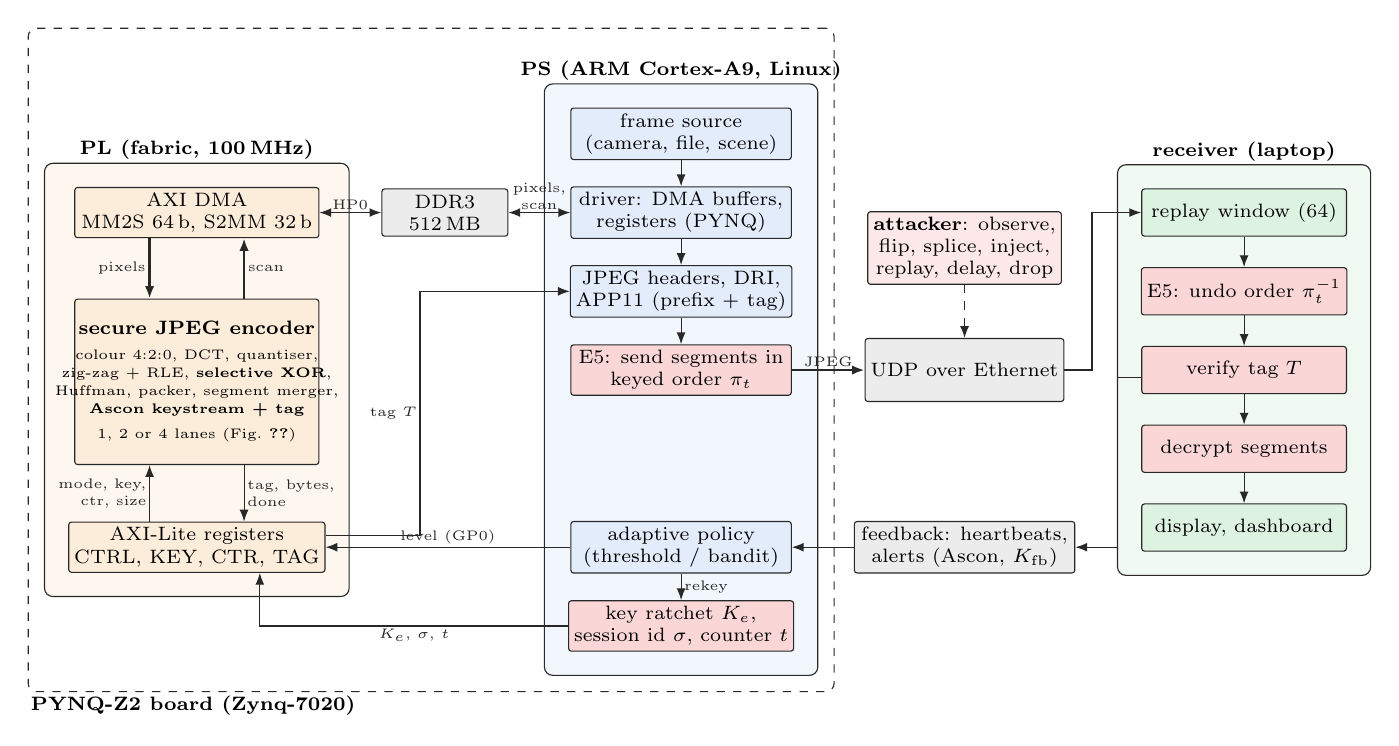
\begin{tikzpicture}[x=1cm, y=1cm]
% ---------------- PL (fabric)
\node[pl, minimum width=31mm] (dma) at (1.6,-0.6) {AXI DMA\\MM2S 64\,b, S2MM 32\,b};
\node[pl, minimum width=31mm, minimum height=21mm] (enc) at (1.6,-2.75) {};
\node[align=center, font=\scriptsize] at (enc.center) {\textbf{secure JPEG encoder}\\[1pt]
  \tiny colour 4:2:0, DCT, quantiser,\\[-1.5pt]\tiny zig-zag + RLE, \textbf{selective XOR},\\[-1.5pt]
  \tiny Huffman, packer, segment merger,\\[-1.5pt]\tiny \textbf{Ascon keystream + tag}\\[1pt]\tiny 1, 2 or 4 lanes (Fig.~\ref{fig:pl})};
\node[pl, minimum width=31mm] (regs) at (1.6,-4.85) {AXI-Lite registers\\CTRL, KEY, CTR, TAG};
\draw[bus] ([xshift=-6mm]dma.south) -- node[lbl, left]{pixels} ([xshift=-6mm]enc.north);
\draw[bus] ([xshift=6mm]enc.north) -- node[lbl, right]{scan} ([xshift=6mm]dma.south);
\draw[arr] ([xshift=-6mm]regs.north) -- node[lbl, left, align=right]{mode, key,\\ctr, size} ([xshift=-6mm]enc.south);
\draw[arr] ([xshift=6mm]enc.south) -- node[lbl, right, align=left]{tag, bytes,\\done} ([xshift=6mm]regs.north);
\begin{scope}[on background layer]
\node[grp, fill=plfill!40, fit=(dma)(enc)(regs), label={[ttl]north:PL (fabric, 100\,MHz)}] (plg) {};
\end{scope}
% ---------------- DDR
\node[blk, fill=netfill, minimum width=16mm] (ddr) at (4.75,-0.6) {DDR3\\512\,MB};
% ---------------- PS (ARM)
\node[arm, minimum width=28mm] (src) at (7.75,0.4)  {frame source\\(camera, file, scene)};
\node[arm, minimum width=28mm] (drv) at (7.75,-0.6) {driver: DMA buffers,\\registers (PYNQ)};
\node[arm, minimum width=28mm] (hdr) at (7.75,-1.6) {JPEG headers, DRI,\\APP11 (prefix + tag)};
\node[cry, minimum width=28mm] (perm) at (7.75,-2.6) {E5: send segments in\\keyed order $\pi_t$};
\node[arm, minimum width=28mm] (pol) at (7.75,-4.85) {adaptive policy\\(threshold / bandit)};
\node[cry, minimum width=28mm] (kr) at (7.75,-5.85) {key ratchet $K_e$,\\session id $\sigma$, counter $t$};
\begin{scope}[on background layer]
\node[grp, fill=psfill!45, fit=(src)(kr), label={[ttl]north:PS (ARM Cortex-A9, Linux)}] (ps) {};
\coordinate (pstop) at ([yshift=5mm]ps.north);
\node[grp, dashed, fit=(plg)(ps)(ddr)(pstop), inner sep=2mm, label={[ttl, anchor=north west]south west:PYNQ-Z2 board (Zynq-7020)}] (board) {};
\end{scope}
\draw[arr] (src) -- (drv); \draw[arr] (drv) -- (hdr); \draw[arr] (hdr) -- (perm);
\draw[darr] (drv.west) -- node[lbl, above, align=center]{pixels,\\scan} (ddr.east);
\draw[darr] (ddr.west) -- node[lbl, above]{HP0} (dma.east);
\draw[arr] (pol.west) -- node[lbl, above]{level (GP0)} (regs.east);
\draw[arr] (kr.west) -| node[lbl, pos=0.25, below]{$K_e$, $\sigma$, $t$} ([xshift=8mm]regs.south);
\draw[arr] ([yshift=1.5mm]regs.east) -- ++(1.2,0) |- node[lbl, pos=0.25, left]{tag $T$} (hdr.west);
\draw[arr] (pol.south) -- node[lbl, right]{rekey} (kr.north);
% ---------------- network
\node[blk, fill=netfill, minimum width=24mm, minimum height=8mm] (net) at (11.35,-2.6) {UDP over Ethernet};
\node[blk, fill=cryfill!55, minimum width=24mm, align=center] (atk) at (11.35,-1.05) {\textbf{attacker}: observe,\\flip, splice, inject,\\replay, delay, drop};
\draw[arr, dashed] (atk) -- (net);
\node[blk, fill=netfill, minimum width=28mm, align=center] (fb) at (11.35,-4.85) {feedback: heartbeats,\\alerts (Ascon, $K_{\mathrm{fb}}$)};
\draw[bus] (perm.east) -- node[lbl, above]{JPEG} (net.west);
\draw[arr] (fb.west) -- (pol.east);
% ---------------- receiver
\node[rx, minimum width=26mm] (rw) at (14.9,-0.6) {replay window (64)};
\node[cry, minimum width=26mm] (unp) at (14.9,-1.6) {E5: undo order $\pi_t^{-1}$};
\node[cry, minimum width=26mm] (tag) at (14.9,-2.6) {verify tag $T$};
\node[cry, minimum width=26mm] (dec) at (14.9,-3.6) {decrypt segments};
\node[rx, minimum width=26mm] (show) at (14.9,-4.6) {display, dashboard};
\begin{scope}[on background layer]
\node[grp, fill=rxfill!45, fit=(rw)(show), label={[ttl]north:receiver (laptop)}] (rxg) {};
\end{scope}
\draw[arr] (rw) -- (unp); \draw[arr] (unp) -- (tag); \draw[arr] (tag) -- (dec); \draw[arr] (dec) -- (show);
\draw[arr] (net.east) -- ++(0.35,0) |- (rw.west);
\draw[arr] (tag.west) ++(0,-0.1) -- ++(-0.3,0) |- (fb.east);
\end{tikzpicture}
}
\caption{System architecture. The fabric (PL) encodes, encrypts and tags; the ARM core (PS) adds headers, reorders E5 segments and runs the key ratchet and policy; the receiver undoes the order, verifies the tag and decrypts, and reports back over an authenticated feedback channel. Shaded red: cryptographic operations.}
\label{fig:system}
\end{figure*}
\begin{figure*}[t]
\centering
\resizebox{\textwidth}{!}{% Fabric datapath of the contract-v3 lane encoder (rtl/secure_jpeg_lanes_top.v, rtl/encoder_lane.v).
% Bus widths are the RTL port widths; module names are the RTL file names.
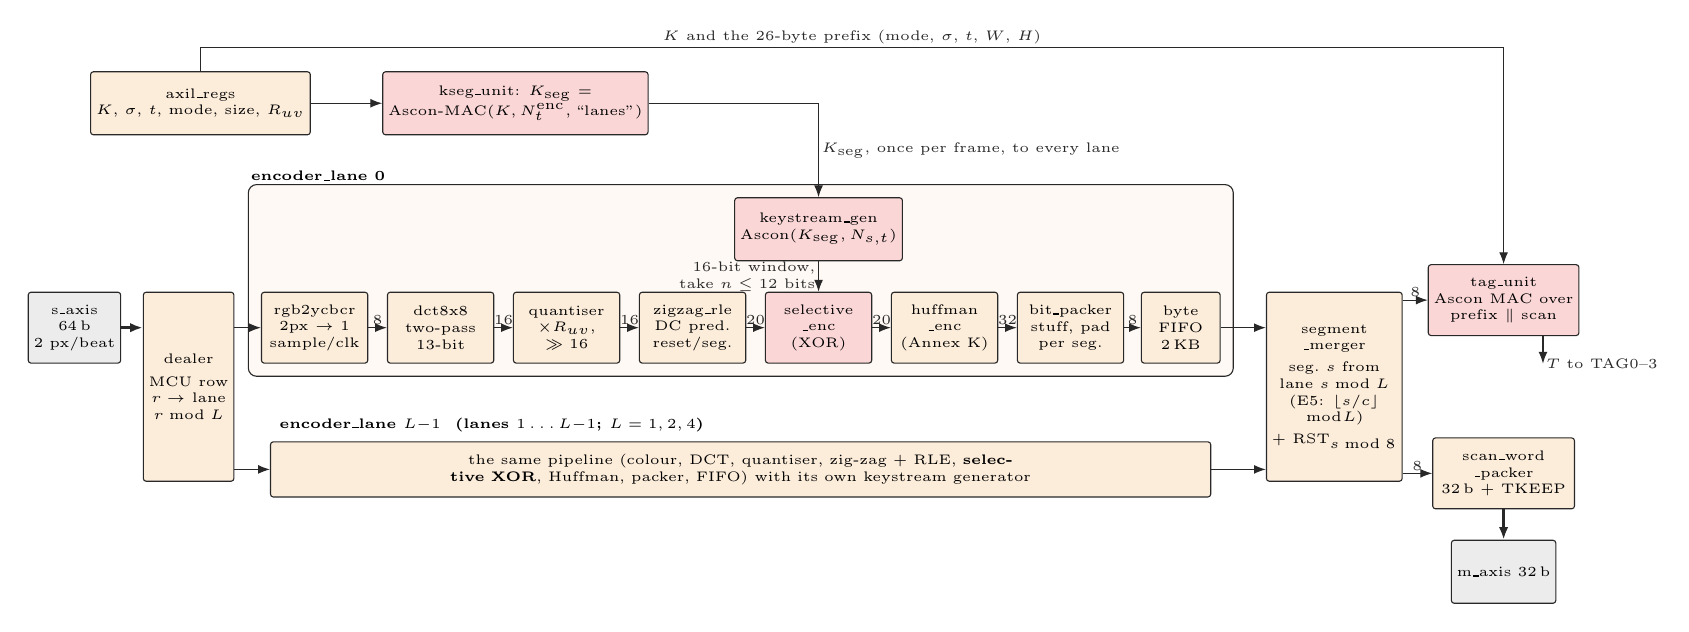
\begin{tikzpicture}[x=1cm, y=1cm, st/.style={pl, minimum height=9mm, minimum width=13.5mm, font=\tiny}]
% ---- input and dealer
\node[blk, fill=netfill, font=\tiny, minimum height=9mm] (in) at (0,0) {s\_axis\\64\,b\\2 px/beat};
\node[pl, font=\tiny, minimum height=24mm, minimum width=11mm, align=center] (deal) at (1.45,-0.75) {dealer\\[2pt]MCU row\\$r\to$ lane\\$r \bmod L$};
\draw[bus] (in) -- (in -| deal.west);
% ---- lane 0 (full) -- y = 0
\node[st] (cc0)  at (3.05,0) {rgb2ycbcr\\2px $\to$ 1\\sample/clk};
\node[st] (dct0) at (4.65,0) {dct8x8\\two-pass\\13-bit};
\node[st] (q0)   at (6.25,0) {quantiser\\$\times R_{uv}$,\\$\gg 16$};
\node[st] (zz0)  at (7.85,0) {zigzag\_rle\\DC pred.\\reset/seg.};
\node[st, fill=cryfill] (se0) at (9.45,0) {selective\\\_enc\\(XOR)};
\node[st] (hu0)  at (11.05,0) {huffman\\\_enc\\(Annex K)};
\node[st] (bp0)  at (12.65,0) {bit\_packer\\stuff, pad\\per seg.};
\node[st, minimum width=10mm] (ff0)  at (14.05,0) {byte\\FIFO\\2\,KB};
\node[cry, font=\tiny, minimum width=19mm, minimum height=8mm] (ks0) at (9.45,1.25) {keystream\_gen\\Ascon$(K_{\mathrm{seg}}, N_{s,t})$};
\draw[arr] (ks0) -- node[lbl, left, align=right]{16-bit window,\\take $n\le 12$ bits} (se0);
\draw[arr] (deal.east |- cc0) -- (cc0);
\draw[arr] (cc0) -- node[lbl, above]{8} (dct0);
\draw[arr] (dct0) -- node[lbl, above]{16} (q0);
\draw[arr] (q0) -- node[lbl, above]{16} (zz0);
\draw[arr] (zz0) -- node[lbl, above]{20} (se0);
\draw[arr] (se0) -- node[lbl, above]{20} (hu0);
\draw[arr] (hu0) -- node[lbl, above]{32} (bp0);
\draw[arr] (bp0) -- node[lbl, above]{8} (ff0);
\begin{scope}[on background layer]
\node[grp, fill=plfill!30, fit=(cc0)(ff0)(ks0), inner sep=1.6mm, label={[font=\tiny\bfseries, anchor=south west, inner sep=1pt]north west:encoder\_lane 0}] (lane0) {};
\end{scope}
% ---- lane L-1 (collapsed) -- y = -1.6
\node[pl, font=\tiny, text width=118mm, minimum height=7mm, align=center] (laneL) at (8.46,-1.8) {the same pipeline (colour, DCT, quantiser, zig-zag + RLE, \textbf{selective XOR}, Huffman, packer, FIFO) with its own keystream generator};
\node[font=\tiny\bfseries, anchor=south west] at (laneL.north west) {encoder\_lane $L{-}1$ \ (lanes $1 \ldots L{-}1$; $L = 1, 2, 4$)};
\draw[arr] (deal.east |- laneL) -- (laneL);
% ---- merger, tag, word packer
\node[pl, font=\tiny, minimum height=24mm, minimum width=13mm, align=center] (mrg) at (16.0,-0.75) {segment\\\_merger\\[2pt]seg.\ $s$ from\\lane $s \bmod L$\\(E5: $\lfloor s/c\rfloor$\\$\bmod L$)\\[2pt]+ RST$_{s \bmod 8}$};
\draw[arr] (ff0.east) -- (ff0.east -| mrg.west);
\draw[arr] (laneL.east) -- (laneL.east -| mrg.west);
\node[cry, font=\tiny, minimum width=18mm, minimum height=9mm] (tag) at (18.15,0.35) {tag\_unit\\Ascon MAC over\\prefix $\|$ scan};
\node[pl, font=\tiny, minimum width=18mm, minimum height=9mm] (wp) at (18.15,-1.85) {scan\_word\\\_packer\\32\,b + TKEEP};
\draw[arr] (mrg.east |- tag) -- node[lbl, above]{8} (tag.west);
\draw[arr] (mrg.east |- wp) -- node[lbl, above]{8} (wp.west);
\node[blk, fill=netfill, font=\tiny, minimum height=8mm] (out) at (18.15,-3.1) {m\_axis 32\,b};
\draw[bus] (wp) -- (out);
% ---- per-frame key, registers
\node[cry, font=\tiny, minimum width=24mm, minimum height=8mm] (kseg) at (5.6,2.85) {kseg\_unit: $K_{\mathrm{seg}}$ =\\Ascon-MAC$(K, N^{\mathrm{enc}}_t, \text{``lanes''})$};
\draw[arr] (kseg.east) -| node[lbl, pos=0.75, right]{$K_{\mathrm{seg}}$, once per frame, to every lane} (ks0.north);
\node[pl, font=\tiny, minimum width=24mm, minimum height=8mm] (regs) at (1.6,2.85) {axil\_regs\\$K$, $\sigma$, $t$, mode, size, $R_{uv}$};
\draw[arr] (regs) -- (kseg);
\draw[arr] (regs.north) -- ++(0,0.3) -| node[lbl, pos=0.25, above]{$K$ and the 26-byte prefix (mode, $\sigma$, $t$, $W$, $H$)} (tag.north);
\draw[arr] (tag.south) ++(0.5,0) -- ++(0,-0.35) node[lbl, right]{$T$ to TAG0--3};
\end{tikzpicture}
}
\caption{Fabric datapath of the lane encoder (\texttt{secure\_jpeg\_lanes\_top}); numbers on arrows are bus widths in bits. MCU row $r$ goes to lane $r \bmod L$; every lane restarts DC prediction and its keystream per restart segment; the merger restores raster order and inserts restart markers; the tag unit authenticates the merged scan.}
\label{fig:pl}
\end{figure*}

\textit{Threat model.} The attacker on the network path observes all traffic and may modify, drop, delay, replay or inject video and feedback datagrams; it holds no key. Sender and receiver share a master key $K_{\mathrm{m}}$ provisioned at installation; key distribution, physical and side-channel attacks are out of scope.

\textit{Encryption inside the entropy coder.} For a quantized coefficient $v \neq 0$ JPEG writes a Huffman code for (run, $s$), $s = \lfloor \log_2 |v| \rfloor + 1$, followed by the $s$-bit field
\begin{equation}
\amp(v) = \begin{cases} v, & v > 0\\ v + 2^s - 1, & v < 0~.\end{cases}
\end{equation}
Given keystream bits $z_0 z_1 \ldots$, a selected symbol is encrypted as
\begin{equation}
\amp' = \amp \xor z_0 (2^s - 1) \xor \alpha \textstyle\sum_{k=1}^{s-1} z_k 2^{k-1},
\label{eq:enc}
\end{equation}
where $\alpha = 1$ if amplitudes are selected. Since $\amp(v) \xor (2^s - 1) = \amp(-v)$, the first term is exactly a sign change; the second changes only the $s-1$ low bits, so $|v|$ stays in $[2^{s-1}, 2^s - 1]$. Hence $s$, the Huffman code and the stream length never change, and the output is a valid JPEG for any key. Fig.~\ref{fig:circuit} shows the gate-level circuit; it consumes $n = [\text{sign}] + \alpha (s - 1) \le 11$ bits per symbol in one clock from a 16-bit window, while the Ascon core delivers 128 bits every 9 cycles, so the cipher never stalls the encoder.

\begin{figure}[t]
\centering
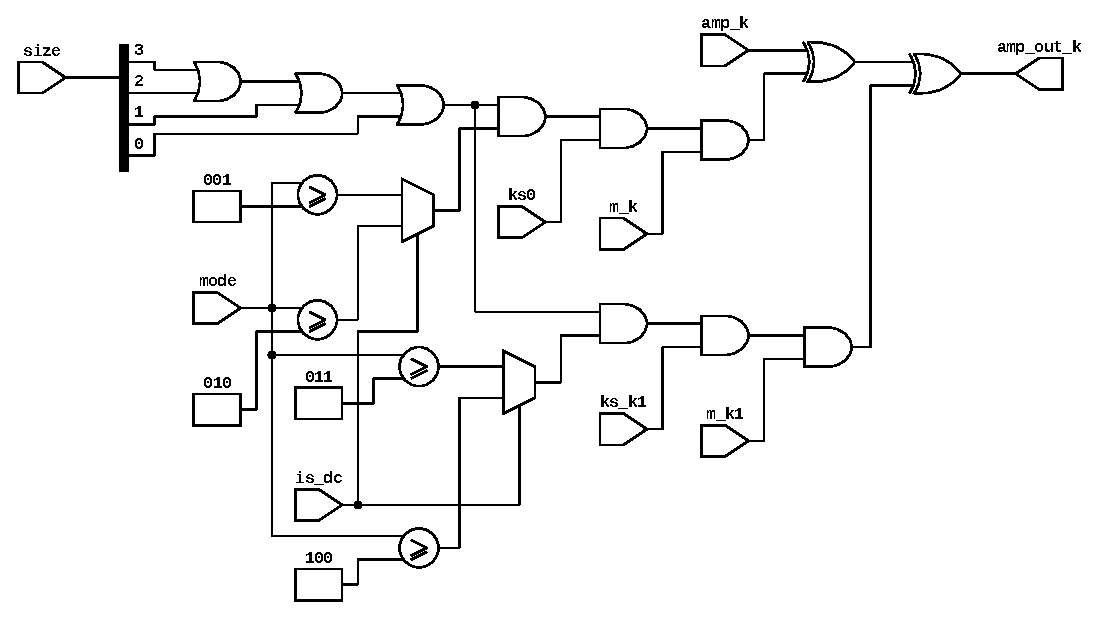
\includegraphics[width=\columnwidth]{figures/fig_selective_enc_bitslice.pdf}
\caption{Gate-level circuit of bit $k$ of the encryption stage, generated from the RTL (Yosys, netlistsvg): the comparators and multiplexers (select: is\_dc) form the sign and amplitude enables, and two XORs apply~\eqref{eq:enc}. $m_k = [k < s]$; ks0, ks\_k1: keystream bits 0 and $k{+}1$. Eleven such slices form the stage.}
\label{fig:circuit}
\end{figure}

\textit{Keys, nonces and tag.} The video key follows a one-way ratchet, $K_{e+1} = \KDF(K_e, \text{ratchet}, e{+}1)$, with $\KDF$ the Ascon tag under a reserved nonce; a separate key $\Kfb$ protects feedback. The 128-bit nonce is $N(\sigma, t, b) = \sigma \cat t \cat b$: a 64-bit session identifier $\sigma$ (48 random bits per boot and a 16-bit epoch), a 63-bit frame counter $t$ and a purpose bit $b$. Each frame derives a segment key and authenticates its scan:
\begin{align}
\Kseg &= \MAC_{K_e}\bigl(N(\sigma, t, 0), \text{``lanes''}\bigr),\\
Z_s &= \Enc_{\Kseg}\bigl(N(s, t, 0), 0^\ell\bigr),\\
T_t &= \MAC_{K_e}\bigl(N(\sigma, t, 1), P_t \cat \text{scan}_t\bigr),
\end{align}
where $Z_s$ is the keystream of restart segment $s$ and $P_t$ is a 26-byte prefix (version, level, $\sigma$, $t$, width, height). Binding the level stops downgrades; $(K, N)$ never repeats because $t$ increases, a rekey changes $K_e$ and $\sigma$, and two boots share $\sigma$ with probability $2^{-48}$ per pair.

\begin{figure}[t]
\centering
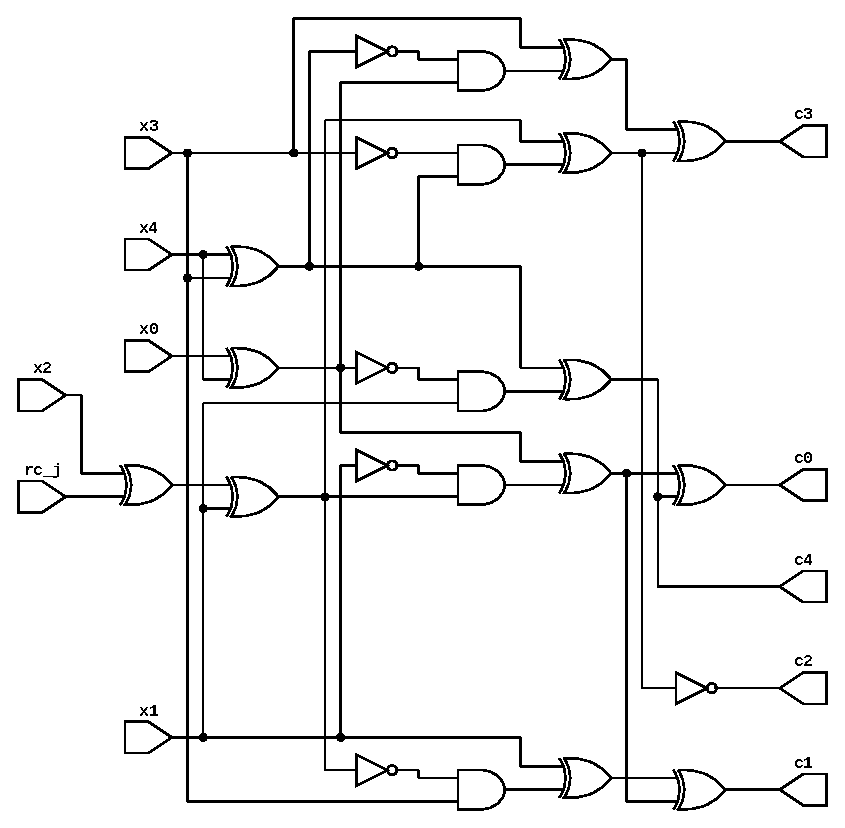
\includegraphics[width=0.92\columnwidth]{figures/fig_ascon_sbox_slice.pdf}
\caption{One of 64 bit slices of the Ascon round in our RTL ($p_C$ and $p_S$), generated from the Verilog: 12 XOR, 5 AND, 6 NOT gates; one round per clock cycle.}
\label{fig:ascon}
\end{figure}

\textit{Protection levels.} E0 only tags; E1 encrypts AC signs, E2 also DC signs (the default floor), E3 AC amplitudes, E4 DC amplitudes. Huffman symbols reveal where non-zero coefficients are, so E1--E4 leak outlines. E5 encrypts like E4 and sends the $M$ macroblocks in a keyed order $\pi_t$ (Fig.~\ref{fig:e5}): Fisher--Yates with rejection sampling on the keystream of $(K_\pi, N(\sigma, t, 0))$ yields a uniform permutation, $\log_2 M! = \PermBitsQVGA$ bits at 320$\times$240 ($M = \McuQVGA$), new in every frame. Each macroblock is a restart segment, so the fabric needs no frame buffer; the ARM only reorders segments and the receiver restores raster order before checking $T_t$, so a moved segment fails the tag.

\begin{figure}[t]
\centering
\resizebox{\columnwidth}{!}{% E5 in hardware form (docs/INTERFACES.md §8.6): fabric codes MCU segments in raster order and tags them,
% (black bars: restart markers, none after the last segment) the ARM sends them in the keyed order pi_t, the receiver restores raster order before the tag check.
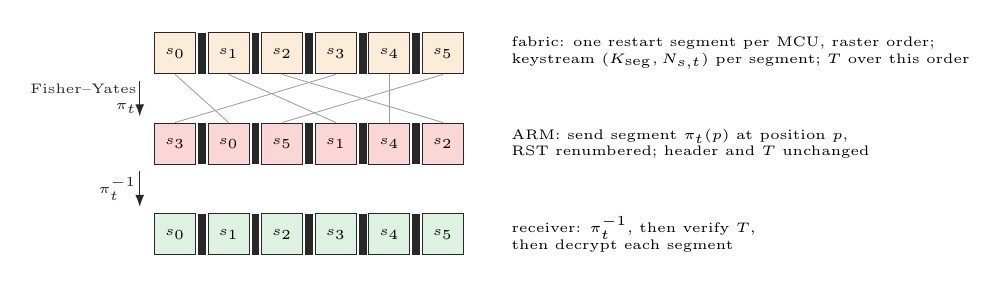
\begin{tikzpicture}[x=1cm, y=1cm,
  seg/.style={draw=inkc, minimum width=5.2mm, minimum height=5.2mm, inner sep=0pt, font=\tiny},
  rst/.style={fill=inkc, minimum width=1.0mm, minimum height=5.2mm, inner sep=0pt},
  st/.style={font=\tiny, align=left, anchor=west}]
\def\segrow#1#2#3{% #1 y, #2 list of labels, #3 fill
  \foreach \l [count=\i from 0] in {#2} {
    \node[seg, fill=#3] at (\i*0.68, #1) {$\l$};
    \ifnum\i<5 \node[rst] at (\i*0.68+0.34, #1) {};\fi
  }}
\segrow{0}{s_0,s_1,s_2,s_3,s_4,s_5}{plfill}
\node[st] at (4.15,0.0) {fabric: one restart segment per MCU, raster order;\\keystream $(K_{\mathrm{seg}}, N_{s,t})$ per segment; $T$ over this order};
\segrow{-1.15}{s_3,s_0,s_5,s_1,s_4,s_2}{cryfill}
\node[st] at (4.15,-1.15) {ARM: send segment $\pi_t(p)$ at position $p$,\\RST renumbered; header and $T$ unchanged};
\segrow{-2.3}{s_0,s_1,s_2,s_3,s_4,s_5}{rxfill}
\node[st] at (4.15,-2.3) {receiver: $\pi_t^{-1}$, then verify $T$,\\then decrypt each segment};
\draw[arr] (-0.45,-0.35) -- node[lbl, left, align=right]{Fisher--Yates\\$\pi_t$} (-0.45,-0.8);
\draw[arr] (-0.45,-1.5) -- node[lbl, left]{$\pi_t^{-1}$} (-0.45,-1.95);
\foreach \a/\b in {0/1,1/3,2/5,3/0,4/4,5/2} {
  \draw[inkc!45, line width=0.3pt] (\a*0.68,-0.27) -- (\b*0.68,-0.88);
}
\end{tikzpicture}
}
\caption{E5 in hardware form: raster-order segments from the fabric, keyed order on the wire, raster order again before the tag check.}
\label{fig:e5}
\end{figure}

\textit{Lanes.} One pipeline takes one sample per clock and 4:2:0 has 1.5 samples per pixel; a 64-bit input brings two pixels per clock. With $L$ lanes the cost per pixel is therefore bounded by
\begin{equation}
c_L \ge \max\!\left(\tfrac{1.5}{L}, \tfrac{1}{2}\right)\ \text{cycles/pixel},\qquad \Theta_L = f_{\mathrm{clk}} / c_L,
\end{equation}
i.e.\ at most \BoundOneMpix, \BoundTwoMpix{} and \BoundFourMpix\,Mpixel/s for $L = 1, 2, 4$ at 100\,MHz. Restart segments make lanes independent (Fig.~\ref{fig:pl}); the bytes do not depend on $L$. Built for a camera's YUYV (4:2:2) input instead, a beat carries four pixels, the colour multipliers disappear and the bound becomes $\max(1.5/L, 1/4)$.

\textit{Feedback and policy.} The receiver checks a 64-frame replay window and returns authenticated heartbeats and alerts. Missing heartbeats for 3\,s raise the top level and rekey (dead-man rule). A threshold policy escalates on tag failures, replays, loss patterns and forged feedback; a contextual bandit is the alternative.

% =====================================================================================================
\section{Implementation and Verification}\label{sec:impl}
A Python golden model passes all 1089 Ascon-AEAD128 known-answer tests; every RTL block has a cocotb testbench with random back-pressure that reports the first mismatch, and the encoders are byte-exact with the model in Icarus and Vivado XSim, for one, two and four lanes and all six levels. Encryption costs no cycles (E0--E4 differ by at most \MaxExtraCycles{} cycles per frame); cycles per pixel follow $1.5 + \FillA/r$ for $r$ MCU rows, \CppVGA{} at 640$\times$480. After place and route the encoder meets \TopMhz\,MHz (WNS $+$\TopWns\,ns): \TopMpix\,Mpixel/s, \FpsVGA{} frames/s at VGA, \TopLuts{} LUTs and about \SaifTopMw\,mW with simulated switching activity (Table~\ref{tab:resources}). Two and four lanes reach \RtlTwoLanesMpix{} and \RtlFourLanesMpix\,Mpixel/s in RTL simulation and close 100\,MHz; E5 costs no BRAM, and with two lanes it draws \SaifLanesEfiveMw\,mW against \SaifLanesEtwoMw\,mW for E2. Out of context one and two lanes also meet 125\,MHz (WNS \TopWnsAtOneTwoFive{} and \LanesTwoWnsAtOneTwoFive\,ns). With YUYV input four lanes reach \YuyvFourLanesMpix\,Mpixel/s and read half the bytes from DDR. All three PYNQ-Z2 systems (Zynq PS, AXI DMA, one, two or four lanes) close timing at 100\,MHz. Each Ascon core (Fig.~\ref{fig:ascon}) takes \AsconLutMin--\AsconLutMax{} LUTs (Table~\ref{tab:compare}).

\begin{figure}[t]
\centering
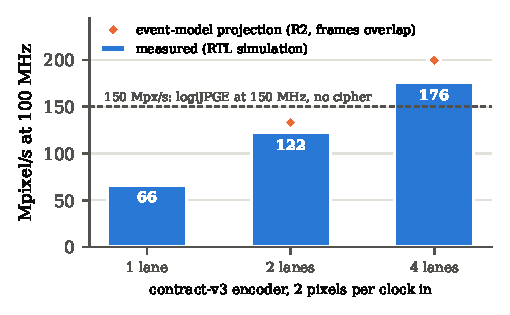
\includegraphics[width=0.92\columnwidth]{figures/fig_lanes_rtl.pdf}
\caption{Lane encoder throughput at 100\,MHz, 640$\times$480, cycle-accurate RTL simulation with every frame bit-exact (bars); diamonds: event-model projection with overlapping frames; dashed: a commercial encoder without cryptography~\cite{logijpge}.}
\label{fig:lanesrtl}
\end{figure}

% generated by paper/make_assets.py from paper/data -- do not edit
\begin{table}[t]
\caption{Resources on the xc7z020 (53\,200 LUT, 106\,400 FF, 140 BRAM36, 220 DSP). Source: Vivado post-route, out of context, 100\,MHz with I/O delays of 20\,\% of the period, WNS +0.630\,ns.}
\label{tab:resources}
\centering\small
\resizebox{\columnwidth}{!}{%
\begin{tabular}{lrrrr}
\toprule
Block & LUT & FF & BRAM36 & DSP \\
\midrule
Encoder (all) & 4785 (9.0\%) & 3051 (2.9\%) & 25.5 (18.2\%) & 23 (10.4\%) \\
\quad colour conversion + line buffers & 459 & 220 & 25 & 0 \\
\quad DCT and quantizer & 806 & 69 & 0 & 22 \\
\quad zig-zag, Huffman, packing & 717 & 323 & 0 & 0 \\
\quad keystream generator (Ascon) & 949 & 851 & 0 & 0 \\
\quad tag unit (Ascon) & 1358 & 1072 & 0 & 0 \\
\quad selective encryption & 82 & 24 & 0 & 0 \\
\quad AXI-Lite registers & 392 & 451 & 0 & 0 \\
\bottomrule
\end{tabular}}
\end{table}

% generated by paper/make_assets.py from paper/data -- do not edit
\begin{table}[t]
\caption{Comparison with published FPGA designs. Their numbers are as reported by each source; ours are
post-route (Table~\ref{tab:resources}) with throughput from the RTL cycle count. Mpx/s: million pixels per second.}
\label{tab:compare}
\centering\small
\resizebox{\columnwidth}{!}{%
\begin{tabular}{llrrrrrl}
\toprule
Design & Device & LUT & BRAM & DSP & MHz & Mpx/s & Crypto \\
\midrule
Ours: encoder & Zynq-7020 & 5{,}039 & 24.5 & 23 & 100 & 61 & sel.\ AEAD \\
Ours: one Ascon & Zynq-7020 & 860--969 & 0 & 0 & 100 & -- & AEAD core \\
logiJPGE~\cite{logijpge} & Zynq-7020 & 3{,}240 & 16 & 30 & 150 & 150 & none \\
CAST JPEG-E-S~\cite{castjpeg} & Artix-7 & 3{,}069 & 2 & 16 & 166 & -- & none \\
Khairallah~\cite{khairallah2023} & Artix-7 & 1{,}031 & 0 & 0 & 200 & -- & MAC \\
Kurian~\cite{kurian2025} & Artix-7 & 5{,}335 & 32 & 0 & 100 & -- & AEAD \\
\bottomrule
\end{tabular}}
\end{table}


% =====================================================================================================
\section{Security Evaluation}\label{sec:security}
\textit{Setup.} We score what a keyless observer can reconstruct: the stream decoded as is, and a \emph{replacement attack} that substitutes fixed guesses for encrypted values. Leakage is the Pearson correlation of Sobel gradient magnitudes with the original (edge correlation, 0: no outline). Sources: a synthetic scene, \NumClips{} private clips, \NumOpenClips{} Blender films and the 24 Kodak images. All levels decode without error in \Decoders.

\begin{figure*}[t]
\centering
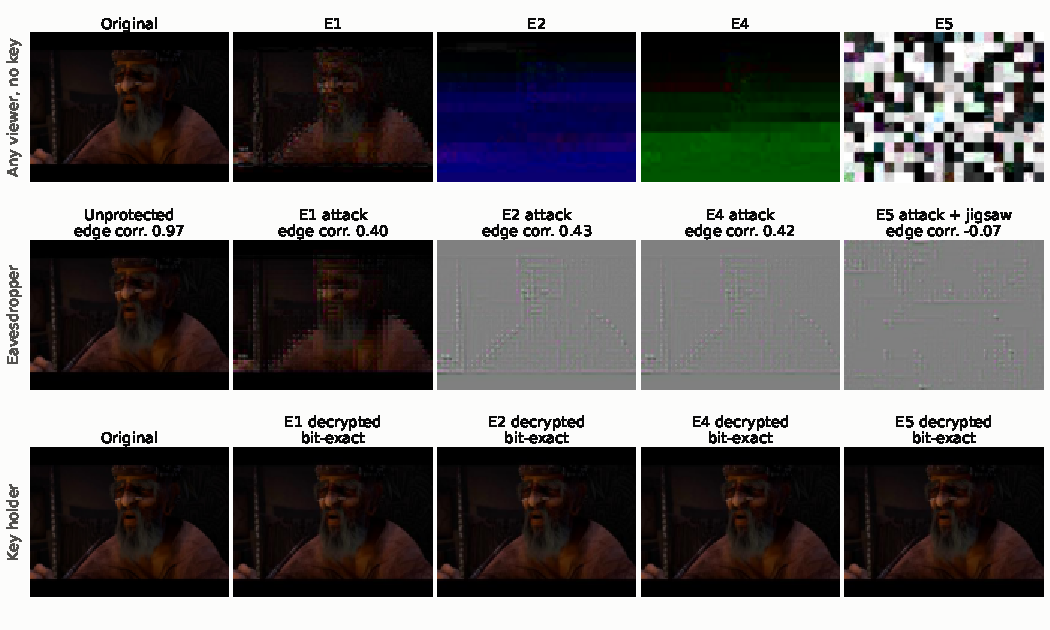
\includegraphics[width=0.62\textwidth]{figures/fig_visual_grid.pdf}
\caption{One frame of the Sintel trailer (\copyright{} Blender Foundation, CC~BY~3.0). Top: any viewer without the key. Middle: the eavesdropper's best picture with its edge correlation (E5: after the jigsaw solver). Bottom: the key holder, bit-exact.}
\label{fig:grid}
\end{figure*}

\textit{Outline leakage.} Under E1--E4 the eavesdropper sees the scene's outline (edge correlation \LeakEOneFourMin--\LeakEOneFourMax, Table~\ref{tab:leakage}, Fig.~\ref{fig:grid}); encrypting amplitudes does not help, because positions and sizes stay public. E5 removes it (\LeakEFiveMin{} to \LeakEFiveMax) for \CostEfive\,\% encrypted bits, against \CostEfour\,\% for E4, at \OverheadEfiveQVGA--\OverheadEfiveVGA\,\% more bytes for the restart markers.

% generated by paper/make_assets.py from paper/data -- do not edit
\begin{table}[t]
\caption{Outline leakage: edge correlation between the original and the eavesdropper's best keyless reconstruction (decode or replacement attack; 0 = no outline), up to 20 frames per source; frames without edges are skipped. The first row is the fraction of payload bits encrypted.}
\label{tab:leakage}
\centering\small\setlength{\tabcolsep}{4pt}
\resizebox{\columnwidth}{!}{%
\begin{tabular}{lrrrrrr}
\toprule
Source & E0 & E1 & E2 & E3 & E4 & E5 \\
\midrule
Enc.\ share & 0.00 & 0.11 & 0.13 & 0.26 & 0.30 & 0.31 \\
\midrule
Synthetic & 1.00 & 0.38 & 0.36 & 0.37 & 0.37 & 0.00 \\
Trailer A & 0.99 & 0.47 & 0.34 & 0.34 & 0.33 & 0.01 \\
Trailer B & 0.99 & 0.58 & 0.27 & 0.31 & 0.30 & 0.02 \\
Talk A & 0.99 & 0.50 & 0.44 & 0.44 & 0.44 & -0.00 \\
Talk B & 0.99 & 0.49 & 0.38 & 0.44 & 0.43 & 0.01 \\
Sintel & 0.99 & 0.35 & 0.25 & 0.26 & 0.27 & -0.00 \\
Tears of Steel & 0.99 & 0.47 & 0.34 & 0.35 & 0.43 & -0.01 \\
Kodak & 0.99 & 0.39 & 0.32 & 0.33 & 0.30 & 0.00 \\
\bottomrule
\end{tabular}}
\end{table}


\textit{Benchmark against published schemes.} We re-implemented four format-compliant schemes~\cite{vandroogenbroeck2002,kishore2015,auer2013,hirose2024} with our keystream and scored all schemes under four attacks on \BenchFrames{} frames of \BenchSources{} sources (Fig.~\ref{fig:bench}): A1 decoding, A2 replacement, A3 non-zero counting (NZCA, \cite{hirose2024}) and A4, which recovers the permutation and keystream bits from one known frame and applies them to the next frames. Every published scheme leaks \BenchPubMin--\BenchPubMax{} under its worst attack; fixed key material falls to A4, including Hirose et al.\ with one block per segment (\BenchHiroseOneCross), although it costs as many bytes as E5. E5, keyed anew per frame, stays at or below \BenchEfiveMax{} in both its model and hardware form.

\begin{figure}[t]
\centering
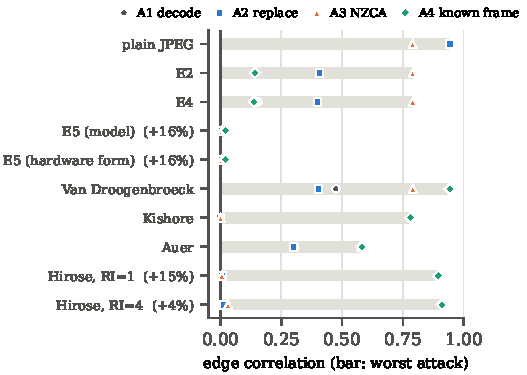
\includegraphics[width=\columnwidth]{figures/fig_bench.pdf}
\caption{SVE-Bench: edge correlation under each attack, pooled over \BenchSources{} sources (byte cost over plain JPEG in brackets when above 2\,\%).}
\label{fig:bench}
\end{figure}

\textit{Stronger attackers.} Greedy and minimum-spanning-tree jigsaw solvers~\cite{pomeranz2011,gallagher2012} place at most \JigsawNeighboursMax{} and \MstNbMax\,\% of E5 neighbours (chance), and one frame's exact permutation places \CpaPlacedEfive\,\% of the next frame's tiles~\cite{li2025shuffle}. The linear program of Lin et al.\ recovers \SrEoneSigns\,\% of E1's signs and \SrEtwoSigns\,\% of E2's (chance 50\,\%). A U-Net~\cite{unet} trained on \LearnBigTrain{} frames and tested on unseen sources breaks E1 (edge \LearnEoneEdge, SSIM \LearnEoneSsim) but learns only brightness and colour under E5 (SSIM \LearnEfiveSsimBig{} against \CtrlTrueSsim{} for a frame-statistics oracle; edge \LearnEfiveEdgeBig, Table~\ref{tab:learned}).

% generated by paper/make_assets.py from paper/data -- do not edit
\begin{table}[t]
\caption{U-Net reconstruction, SSIM / edge corr.\ on unseen test clips. P1: Trailer A$\rightarrow$B, P2: Talk A$\rightarrow$B, P3: Sintel$\rightarrow$Tears of Steel, P4: three clips$\rightarrow$three others. Repl.: replacement attack, P4 test set.}
\label{tab:learned}
\centering\small\setlength{\tabcolsep}{3pt}
\resizebox{\columnwidth}{!}{%
\begin{tabular}{llcccc}
\toprule
Mode & Repl. & P1 & P2 & P3 & P4 \\
\midrule
E1 & 0.55 / 0.40 & 0.72 / 0.53 & 0.70 / 0.66 & 0.55 / 0.42 & 0.79 / 0.69 \\
E2 & 0.17 / 0.40 & 0.42 / 0.33 & 0.27 / 0.34 & 0.13 / 0.32 & 0.34 / 0.40 \\
E4 & 0.18 / 0.39 & 0.43 / 0.34 & 0.28 / 0.32 & 0.12 / 0.26 & 0.35 / 0.40 \\
E5 & 0.14 / 0.00 & 0.34 / -0.02 & 0.26 / 0.02 & 0.22 / 0.00 & 0.36 / 0.04 \\
\bottomrule
\end{tabular}}
\end{table}


% =====================================================================================================
\section{Protocol and Defence Evaluation}\label{sec:protocol}
Sender, network channel with attacker and receiver run as separate processes over UDP (320$\times$240, 10 frames/s). Eleven attacks run 25\,s apart: scan bit flips, mode downgrade, splicing, injection, replay, delay, dropping, junk flood, and dropping, forging or replaying feedback. Over \SuiteRuns{} runs all were mitigated, on average \TtmMean{}\,$\pm$\,\TtmSd\,s after they began, with \SuiteFalse{} false alarms (Table~\ref{tab:attacks}); integrity attacks are caught at the first frame, attacks by absence only by timeouts (dropped feedback, \FbDropTtm\,s). Benign loss up to 6\,\%, delay and reordering raised no alarm (\BenignFalse{} windows). The bandit encrypts \PolCostSave\,\% fewer bits than the threshold rule but reacts later (\PolTtmB{} against \PolTtmT\,s).

% generated by paper/make_assets.py from paper/data -- do not edit
\begin{table}[t]
\caption{Reaction to each active attack (full suite, threshold policy, 3 runs; mean\,$\pm$\,s.d. in seconds). ``First rejection'' is when the receiver first discards a frame; ``mitigated'' is when the sender has raised protection or rekeyed.}
\label{tab:attacks}
\centering\small\setlength{\tabcolsep}{4pt}
\resizebox{\columnwidth}{!}{%
\begin{tabular}{lccc}
\toprule
Attack & Mitigated & First rejection & Mitigated after \\
\midrule
bit flips in the scan & 3/3 & 0.09\,$\pm$\,0.03 & 0.41\,$\pm$\,0.02 \\
mode downgrade in header & 3/3 & 0.06\,$\pm$\,0.02 & 0.44\,$\pm$\,0.02 \\
splice of two frames & 3/3 & 0.13\,$\pm$\,0.00 & 0.46\,$\pm$\,0.01 \\
forged frame injection & 3/3 & 0.14\,$\pm$\,0.06 & 0.44\,$\pm$\,0.03 \\
frame replay & 3/3 & 0.07\,$\pm$\,0.05 & 0.46\,$\pm$\,0.03 \\
frame delay & 3/3 & 4.13\,$\pm$\,0.04 & 1.46\,$\pm$\,0.03 \\
frame dropping & 3/3 & -- & 1.46\,$\pm$\,0.03 \\
junk flood & 3/3 & -- & 0.49\,$\pm$\,0.04 \\
feedback dropping & 3/3 & -- & 3.47\,$\pm$\,0.05 \\
forged feedback & 3/3 & -- & 0.46\,$\pm$\,0.04 \\
feedback replay & 3/3 & -- & 0.44\,$\pm$\,0.01 \\
\bottomrule
\end{tabular}}
\end{table}


% =====================================================================================================
\section{Limitations and Conclusion}
On the PYNQ-Z2 the two-lane E5 bitstream is bit-exact with the golden model in \BoardModes{} at \BoardSizes{} (\BoardFramesTotal{} frames). A 640$\times$480 frame takes \BoardMsVGA\,ms with our Python driver (\BoardFpsVGA{} frames/s; \BoardFpsQVGA{} at 320$\times$240), the same in every level within \BoardSpreadMsVGA\,ms, so encryption costs no time on silicon either; this is the ARM's pixel copy, not the fabric (\RtlTwoLanesVgaMs\,ms in RTL). Board power and the ARM baseline are pending \TODO{GUIDE.md A3, A4}, so our power figures come from simulated switching activity. No level hides frame sizes: ten sizes identify one of \FpVideos{} videos \FpEtwoTen\,\% of the time under E2 (\FpEfiveTen\,\% under E5), and only constant-size frames prevent it, at up to $+$\PadFilmMax\,\% bytes on edited clips. The link can pad every frame to the largest size so far, in comment segments that decoders skip and the tag need not cover. Our attackers are greedy or trained on few clips. The pre-shared key only authenticates a hybrid ML-KEM-768 + X25519 exchange~\cite{fips203} on the ARM, so a recorded session stays secret if that key leaks later or the elliptic curve falls to a quantum computer; Ascon's 128-bit key keeps about $2^{64}$ against Grover's search~\cite{grover1996}.

Encrypting coefficient fields with Ascon inside a JPEG encoder costs no cycles, keeps every level playable and, with a per-frame tag, turns MJPEG into an authenticated stream. Published format-compliant schemes fall to non-zero counting or one known frame; a per-frame keyed shuffle of restart segments, built in hardware without a frame buffer, does not.

\section*{Acknowledgment}
We thank Dr.~Chetana~G for her guidance. \TODO{AI-assistance disclosure as required by the conference.}

\bibliographystyle{IEEEtran}
\bibliography{refs}
\end{document}
